\documentclass{article}


\usepackage[utf8]{inputenc}		% for special characters
\usepackage[english]{babel}
%\usepackage[T1]{fontenc}		% for correct use of western european characterfonts
\usepackage{amsmath}
\usepackage{bm}
\usepackage{natbib}
\usepackage{amssymb}
\usepackage{bbm}

\usepackage{titling}


\usepackage{graphicx}


\usepackage{algorithm}
\usepackage{algpseudocode}
% \usepackage{algorithm}
% keine "End"-Statements in Algorithmen
\algtext*{EndWhile}
\algtext*{EndIf}
\algtext*{EndFor}
\algtext*{EndProcedure}
\algtext*{EndFunction}



\usepackage{caption}
\DeclareCaptionType{code}[Code Listing][List of Code Listings] 

\usepackage{listings}
\usepackage{color}
\definecolor{matlabgreen}{RGB}{28,172,0}
\definecolor{matlabpurple}{RGB}{170,55,241}	
	
\lstset{language=Matlab,
	breaklines=true,
	keywordstyle=\color{blue},
	identifierstyle=\color{black},
	stringstyle=\color{matlabpurple},
	commentstyle=\color{matlabgreen},
	showstringspaces=false,
	numbers=left,
	numberstyle={\color{black}},
	numbersep=9pt
}



\newcommand{\norm}[1]{\left\lVert#1\right\rVert}


\setlength{\parskip}{\baselineskip}
%\setlength{\parindent}{0pt}%

%\setlength{\parindent}{2em}
%\setlength{\parskip}{1em}
%\renewcommand{\baselinestretch}{1.5}


\begin{document}

\title{Kernel Density Estimates and Mean-Shift Clustering}
\author{Jonas Spinner\thanks{jonas.spinner@student.kit.edu} \enspace -- 1927895\\
	Analytics and Statistics\\
	KIT -- Karlsruhe Institute of Technologie}
\date{\today}
\maketitle

\newpage

\tableofcontents

\newpage

\listoffigures

\listoftables

\listofalgorithms

%\lstlistoflistings
\listofcodes


\newpage


\begin{abstract}
	In this seminar paper we are describing and evaluating the mean shift algorithm. It is a nonparametric clustering method which does not depend on prior knowledge on the number and shape of the clusters.
	
	The clusters are defined by the modes of the data density and a iteration procedure is used to let a point converge to its cluster centroid. We introduce the kernel density estimate for estimating the data density and then derive the mean shift algorithm from it.
	
	After presenting the methods we also present different applications of the algorithm, mainly its use in image segmentation.
\end{abstract}

\section{Introduction}

In this seminar paper I am going to discuss the method of kernel density estimation (KDE) and it's use in the mean-shift clustering algorithm (MSC). Clustering is one of the main tasks in Machine-Learning and MSC has many applications, mainly in image segmentation. The mean-shift algorithm is an non-parametric approach which allows a wide range of data distributions without imposing prior knowledge.

The content of this seminar paper is mainly based on \cite{Comaniciu.2002}.

\textbf{History}

The mean shift algorithm was introduced in \cite{Fukunaga.1975} where also the term ``mean shift'' was established. \cite{Comaniciu.2002} and \cite{Comaniciu.2003} are responsible for a gain in interest for the algorithm. These publication popularized the use of the algorithm in image segmenation and tracking.


\textbf{Notation}

In this paper I'm going to use the following conventions. Bold symbols $\bm{x}$ denotes a vector. $\{ \bm{x}_i \}_{i=1}^n$ denotes $n$ samples $\bm{x}_i$, indexed by $i$. $d$ is the dimensionality of the samples. $K(\cdot)$ is a multivariate kernel function $\mathbb{R}^d \rightarrow \mathbb{R}$ and $k(\cdot)$ denotes a single variable kernel function $\mathbb{R} \rightarrow \mathbb{R}$.


\section{Kernel Density Estimation}

In this section we are going to introduce the kernel density estimate. It will be used in the derivation of the mean shift algorithm.

\begin{figure}
	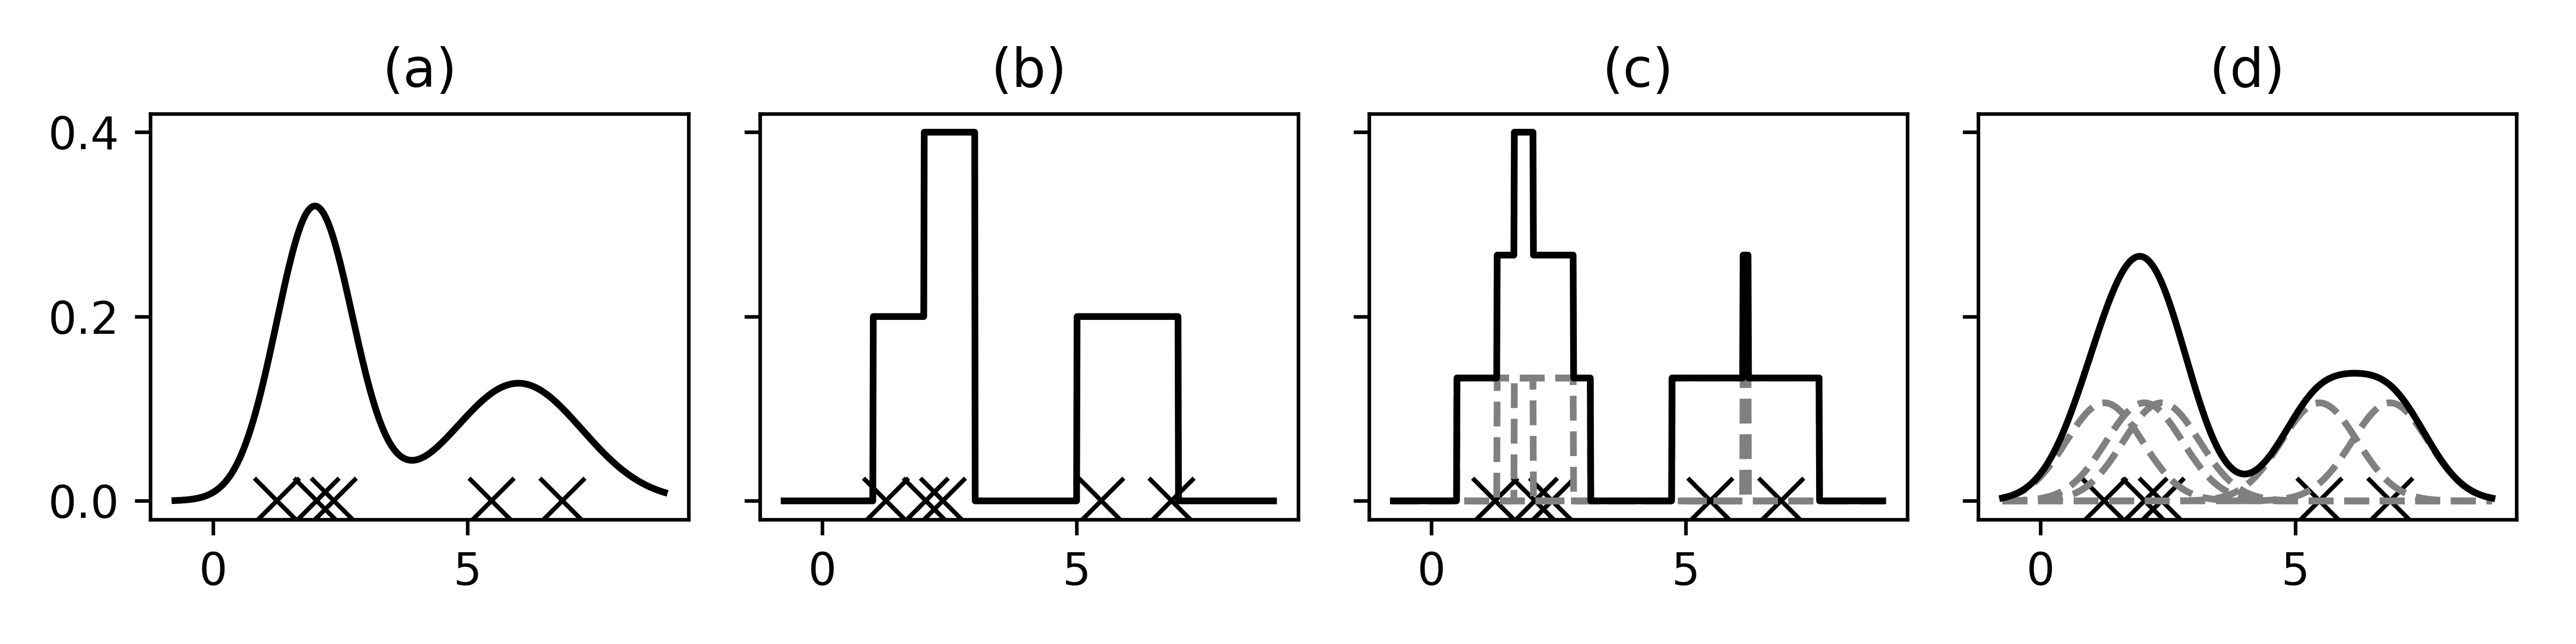
\includegraphics[width=\textwidth]{figures/kde-kernel-density-estimates}
	\caption[Samples, histogram and kernel density estimates]{Samples, histogram and kernel density estimates. Author's illustration.
		(a) The probability density distribution $p(x) = \frac{3}{5} N(x; 2, 0.75^2) + \frac{2}{5} N(x; 6, 1.25^2)$ and five samples drawn from it.
		(b) A histogram with bins $[i,i+1)$, $i \in \mathbb{Z}$.
		(c) A kernel density estimate with a uniform kernel and bandwidth $h=0.75$, $k(x) = \frac{1}{2h}$ for $\lvert x \rvert \leq h$ and $0$ else.
		(d) A kernel density estimate with a gaussian kernel and bandwidth $h=0.75$, $k(x) = \frac{1}{h} \frac{1}{\sqrt{2\pi}} \exp(-\frac{1}{2} \lvert \frac{x}{h} \rvert^2)$.
	}
	\label{fig:kde-kernel-density-estimates}
\end{figure}

% Some methods and algorithms require a probability density function (pdf) of the distribution but only samples are available.

We assume that we have $n$ data points $\{\bm{x}_i\}_{i=1}^n \subset \mathbb{R}^d$, which are independently, identically distributed samples from a unknown probabiltiy distribution $p(\bm{x})$, $\bm{x}_i \overset{i.i.d.}{\sim} p(\cdot)$. We call the corresponding density function $f$. 

The goal of density estimation is estimating the probality density of $p$, given samples $\{\bm{x}_i\}_{i=1}^n$ in $\mathbb{R}^d$, $\bm{x} \sim p(\bm{x})$.


Histograms estimate the probability distribution by bucketing the samples and counting the proportion of samples which fall in each bucket.

The \textbf{kernel density estimate} is defined as

\begin{equation}
	\hat{f}(\bm{x}) = \frac{1}{nh^d} \sum_{i=1}^n K\left(\frac{\bm{x} - \bm{x}_i}{h} \right) \qquad \bm{x} \in \mathbb{R}^d\text{,}
	\label{eq:kernel-density-estimate}
\end{equation}

where $n$ is the sample size, $d$ is the dimensionality of the data, $K(\bm{x})$ is a kernel function and $h$ is a bandwidth parameter. The estimate is dependent on the choice of the kernel function and the bandwidth.

A \textbf{kernel function} $K(\bm{x})$ is a function that satisfies $K(\bm{x}) \geq 0$ and $\int_{\mathbb{R}^d} K(\bm{x}) d\bm{x} =\nobreak 1$. These restrictions on the kernel ensure that $\hat{f}(\bm{x})$ is a valid density. The \textbf{bandwidth} $h$ controls the smoothness of the kernel density estimate. We are going to discuss the choices for kernel functions and the bandwidth in the next section.

The kernel density estimate can be interpreted as the sum of ``bumps'' centered on each data point.

For non-negative kernels, one can see that $\hat{f}(\bm{x})$ is a valid probability density.


\subsection{Other methods}

Another method for estimating a probability density function are histograms. The samples $\{ \bm{x}_i \}_{i=1}^n$ are put into distinct buckets $b_j \subseteq \mathbb{R}^d$ and the probability is estimated by the sample frequency $p(j) = \lvert \{\bm{x}_i \mid \bm{x}_i \in b_j\} / n$ for each bucket.


\subsection{Popular Kernels}

% Kernels:
% uniform, triangular, biweight, triweight, Epanechnikov, normal, and others

% Estimators:
% Nadaraya-Watson kernel-weighted average

\begin{figure}
	\centering
	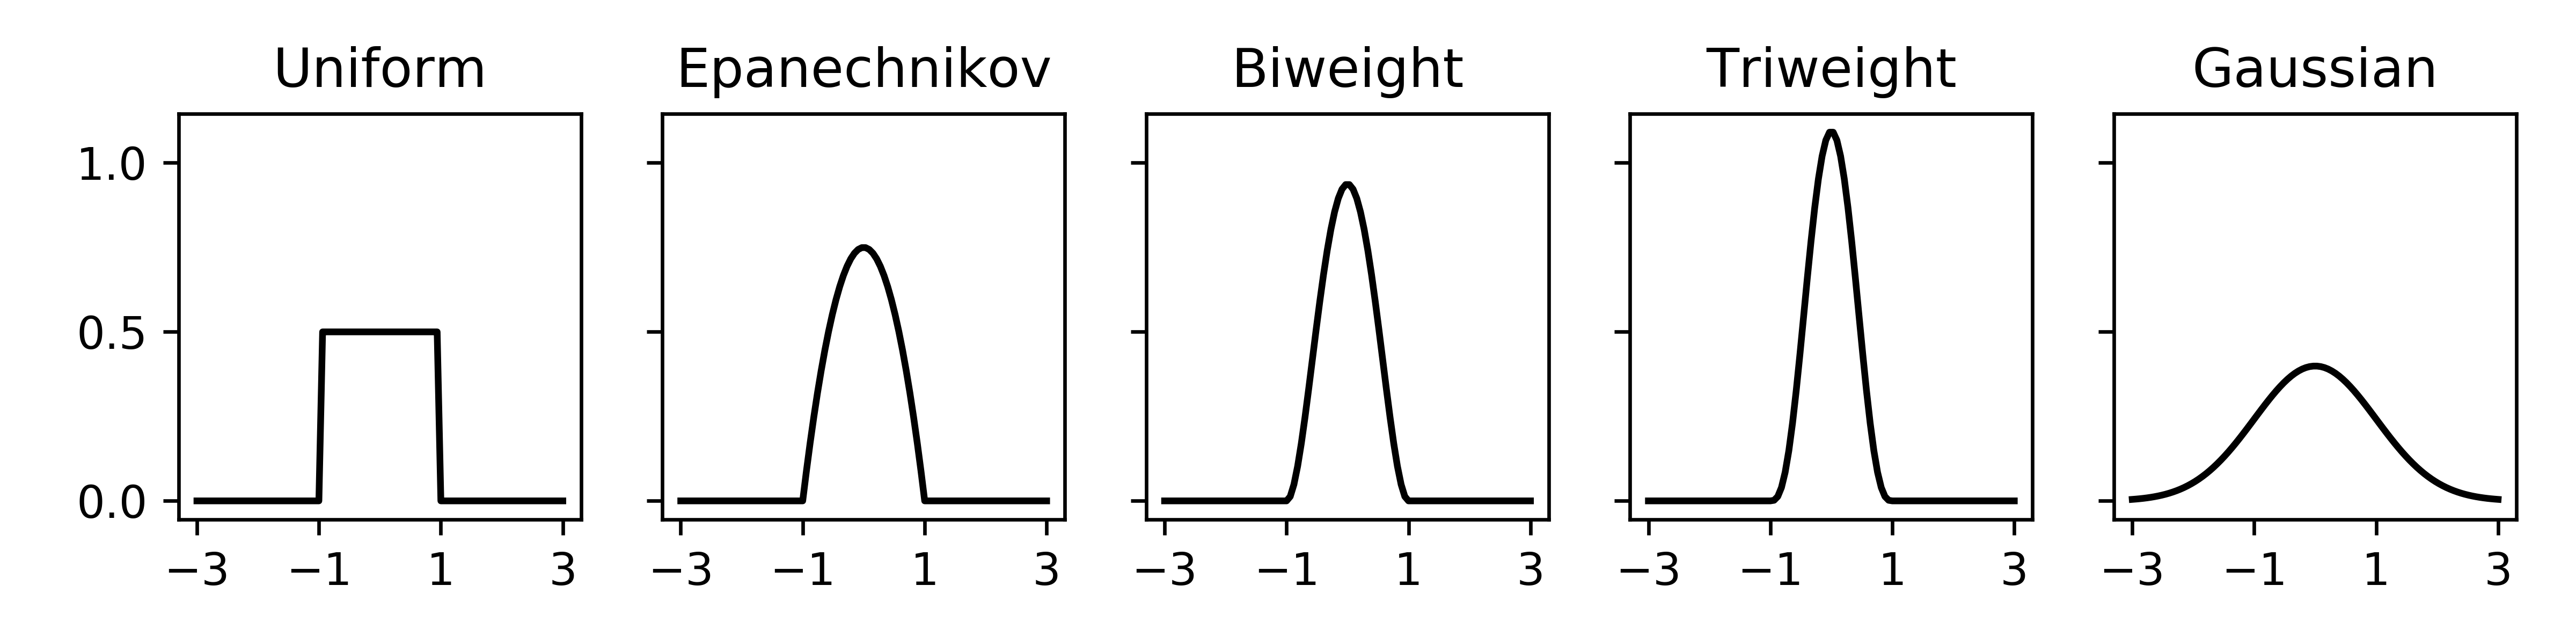
\includegraphics[width=\textwidth]{figures/kde-popular-kernels}
	\caption[Popular kernels]{Popular kernels. Author's illustration. The first four kernels all have support $[-1, 1]$. The gaussian kernel has the support $(-\infty, \infty)$.}
	\label{fig:kde-popular-kernels}
\end{figure}

A general Kernel is a function $K : \mathbb{R}^d \rightarrow \mathbb{R}$ satisfying the following properties. See \citep{Comaniciu.2002} and \citep[p.~95]{Wand.1995}.

\begin{align*}
	\int_{\mathbb{R}^d} K(\bm{x})\mathrm{d}\bm{x} &= 1 \qquad \int_{\mathbb{R}^d} \bm{x} K(\bm{x})\mathrm{d}\bm{x} = \bm{0} \\
	\lim_{\norm{\bm{x}} \rightarrow \infty}  \norm{\bm{x}}^d K(\bm{x})\mathrm{d}\bm{x} &= 0 \qquad \int_{\mathbb{R}^d} \bm{x} \bm{x}^T K(\bm{x})\mathrm{d}\bm{x} = c_K \bm{I}
\end{align*}

\begin{align*}
	K^P(\bm{x}) = \prod_{j=1}^d k(x_j) & \qquad
	K^S(\bm{x}) = a_{k,d} k(\norm{\bm{x}})
\end{align*}

Although there a many kernel functions, we are going to concentrate us on one class of functions: \textbf{radially symmetric kernels}. They are the kernels which can be formulated as

\begin{equation}
	K(\bm{x}) = c_{k,d} k(\norm{\bm{x}}^2)\text{,}
\end{equation}

where $k : [0, \infty]) \rightarrow [0, \infty)$ is called the \textbf{profile} of $K$, and $c_{k,d}$ is a constant which ensures, that $K(\bm{x})$ integrate to 1.

The derivation of the mean shift algorithm is going to be easier and nearly all popular kernels already belong to this class. The most popular kernels for mean shift clustering are the uniform, Epanechnikov and the Gaussian kernel. We are going to shortly introduce them and their profile.

The \textbf{uniform kernel} is defined as being constant in the unit hypersphere and can be written as
\begin{equation}
	K_U(\bm{x}) = \begin{cases}
		\text{vol}(S_d)^{-1} & \text{for} \norm{\bm{x}} \leq 1\\
		0 & \text{else}
	\end{cases}\text{,}
\end{equation}
where $\text{vol}(S_d) = \pi^{d/2}\Gamma((d+2)/2)^{-1}$ is the volume of the d-dimensional hypersphere with $\Gamma(\cdot)$ being the gamma function. If $d=1$ then $\text{vol}(S_d)=2$. The corresponding profile $k_U$ is
\begin{equation}
	k_U(u) = \begin{cases}
		1 & \text{for } 0 \leq u \leq 1\\
		0 & \text{for } 1 < u\text{.}
	\end{cases}
\end{equation}

The \textbf{Epanechnikov kernel} is defined as
\begin{equation}
	K_E(\bm{x}) = \begin{cases}
		\frac{2 + d}{2 \text{vol}(S_d)} (1 - \norm{\bm{x}}^2) & \text{for } \norm{\bm{x}} \leq 1\\
		0 & \text{else}
	\end{cases}
\end{equation}
and its profile $k_E$ is
\begin{equation}
	k_E(u) = \begin{cases}
		1 - u & \text{for } 0 \leq u \leq 1\\
		0 & \text{for } 1 < u\text{.}
	\end{cases}
\end{equation}

The \textbf{gaussian kernel} is defined as
\begin{equation}
	K_G(\bm{x}) = (2 \pi)^{-d/2} \exp\left(-\frac{1}{2} \norm{\bm{x}}^2\right)
\end{equation}
and its profile $k_G$ is
\begin{equation}
	k_G(u) = \exp\left(-\frac{1}{2}u\right)\text{.}
\end{equation}


\begin{table}
	\centering
	\begin{tabular}{lllll}
		Name & Profile support & $k(u)$ & $-k'(u)$ & $K(\bm{x})$ \\ \hline
		Uniform & $u \in [0, 1]$ & $1$ & $0$ & $\text{vol}(S_d)^{-1}$ \\
		Epanechnikov & $u \in [0, 1]$ & $1 - u$ & $1$ & $\frac{1}{2} \text{vol}(S_d)^{-1} (d+2) \left(1 - \norm{\bm{x}}^2\right)$\\
		Biweight & $u \in [0, 1]$ & $(1 - u)^2$ & $2 (1 - u)$ & $\propto \left(1 - \norm{\bm{x}}^2\right)^2$ \\
		Triweight & $u \in [0, 1]$ & $(1 - u)^3$ & $3 (1 - u)^2$ & $\propto \left(1 - \norm{\bm{x}}^2\right)^3$ \\
		Gaussian & $u \in [0, \infty)$ & $\exp\left(-\frac{1}{2}u\right)$ & $\frac{1}{2}\exp\left(-\frac{1}{2}u\right)$ & $(2\pi)^{-d/2} \exp\left(-\frac{1}{2}\norm{\bm{x}}^2\right)$
	\end{tabular}
	\caption[Popular kernel functions]{Popular kernel functions. The kernel functions listed here are all radially symmetric kernels. By looking at the profiles $k(u)$ and the negated derivative $-k'(u)$ we can see the corresponding shadows (see section \ref{sec:mean-shift-vector-properties}). $\text{vol}(S_d)$ is the volume of a $d$-dimensional hypershere and the normalization constants for the biweight and triweight kernels are omitted.}
	\label{tab:popular-kernel-functions}
\end{table}


\subsection{Bandwidth Selection}

One of the main challenges in using the kernel density estimate in practice is the choice of the bandwidth. The univariate case has a rich theoretical background, but the multivariate case is more problematic. \citep[section 3.1]{Comaniciu.2002} lists some general approaches for bandwidth selection.

\begin{itemize}
	\item The stability of the clustering in respect to the bandwidth parameter $h$ is analysed. The number of resulting clusters $K$ is stated as a function of the bandwidth, $K(h)$. Then the midpoint of the largest range for which $K(h)$ stays constant is chosen.
	\item Some objective function is used for evaluating the clustering quality. The bandwidth which maximizes the objective function is chosen.
	\item When the desired number of clusters is known, the bandwidth can be varied to accomplished the desired number. This approach can be modified to ignore smaller clusters.
	\item Another approach is to estimate the bandwidth by the mean $K$ nearest neighbor distance between the data points. $K$ is set to be a percentage of the whole dataset, for example 30 \%. The Python library scikit-learn from \cite{Pedregosa.2011} implements this approach in the method \texttt{estimate\_bandwidth}. In section \ref{sec:application} we implement this method in Matlab and use it in our experiments. The code can be found in Code Listing \ref{code:estimate_bandwidth}.
\end{itemize}

\begin{equation}
\hat{f}_{-i}(\bm{x}) = \frac{1}{(n - 1)h^d} \sum_{j \neq j} K\left(\frac{\bm{x}_j - \bm{x}_j}{h} \right) \qquad \bm{x} \in \mathbb{R}^d
\end{equation}

\begin{align}
\text{MLCV}(h) &= \frac{1}{n} \sum_{i=1}^n \log \hat{f}_{-i}(\bm{x}_i) \\
&= \frac{1}{n} \sum_{i=1}^n \log \left(\sum_{j \neq j}^n K\left(\frac{\bm{x}_j - \bm{x}_j}{h} \right)\right) - \log(n - 1) - d \log(h)
\end{align}





\section{Mean Shift Clustering}

Clustering is one of the main machine learning tasks, concerned with grouping objects $\{x_i\}_{i=1}^n$ into clusters $C_j$ resulting in a clustering $\{ C_j \}_{j=1}^K$.

\subsection{Clustering algorithms}

\textit{introduction}

What does define a good clustering? One can try to minimize a global criterion like $J = \sum_{j=1}^K \sum_{\bm{x}_i \in C_j} \norm{\bm{x}_i - \bm{m}_j}^2$, like the $K$-Means algorithm, or minimize the intra-cluster min, max or average distances between the data points, like in hierarchical clustering. The notion of a ``good'' clustering brings rise to many different clustering algorithms.

Another criteria to differentiate clustering algorithms, are the assumptions that it makes on the data. $K$-Means assumes the data is separable into $K$ clusters. 

There are many different notions of what defines a good clustering and what shapes a cluster can take. These different notions result in different clustering algorithms. One class of clustering algorithms is centroid based clustering. Each cluster is represented by a representative called centroid. For example the representative of a $K$-Means clustering is the mean of the cluster $m_j := \frac{1}{\lvert C_j \rvert} \sum_{x_i \in C_j} x_i$.

\textit{centroid based}

A common concept for several algorithms are \textbf{centroids}. A centroid is a point in the data space, which is a representative for a cluster. $K$-Means defines its centroids as the cluster mean $\bm{m}_j = \frac{1}{\lvert C_j \rvert} \sum_{\bm{x}_i \in C_j} \bm{x}_i$. A shortcoming of this definition is that the cluster mean is not guaranteed to ``look like'' a typical data object.

The mean shift algorithm defines its cluster representatives by the modes of the data density. This definition solves several of shortcomings of other algorithms. The algorithm does not make prior assum


Another way clustering algorithms can be differentiated is whether of not the amount of clusters is given as an input to the algorithm or not. For example the $K$-Means algorithm searches for exactly $K$ clusters. But there are also other notions of a cluster center or representative. One is the added restriction, that the center is itself a data object or atleast ``looks like'' one. The latter is covered by using representatives which are likely also a data object. That's the core of the mean shift clustering algorithm. It estimates the underlying density of the data objects and searches for points which high relative probability. Or in other words it identifies the modes of the estimated density.


\subsection{Density gradient estimation} \label{sec:density-gradient-estimation}

Before we look at the specifics of the mean shift algorithm in section \ref{sec:mean-shift-algorithm}, we look at an estimation of the density gradient and derive the mean shift vector. This section is based on \cite{Comaniciu.2002} and follows its notation.

By defining clusters with the modes of a density function the clustering task becomes a mode finding task where we search for $\bm{x}$ where the density gradient is zero, $\nabla f(\bm{x}) = 0$. As we have no knowledge about the real density $f(\bm{x})$, we have to use an estimate. Recall that the kernel density estimate is defined as
\begin{equation}
	\hat{f}(\bm{x}) = \frac{1}{nh^d} \sum_{i=1}^n K\left(\frac{\bm{x} - \bm{x}_i}{h} \right)\text{.}
	\label{eq:kernel-density-estimate-2}
\end{equation}

We estimate the density gradient $\nabla f(\bm{x})$ by the gradient of the density estimate. Formally we write
\begin{equation}
	\hat\nabla f(\bm{x}) \equiv \nabla \hat{f}(\bm{x}) = \frac{1}{nh^d} \sum_{i=1}^n \nabla K\left(\frac{\bm{x} - \bm{x}_i}{h} \right)\text{.}
	\label{eq:kernel-density-gradient-estimate}
\end{equation}

For simplification we are going to concentrate on the class of \textbf{radially symmetric kernels}. These can be written as
\begin{equation}
	K(\bm{x}) = c_{k,d} k(\norm{\bm{x}}^2)
\end{equation}

where $k : [0, \infty]) \rightarrow [0, \infty)$ is called the \textbf{profile} of $K$, and $c_{k,d}$ is a constant which ensures that $K(\bm{x})$ integrate to $1$. The most common kernels belong to this class of functions.

Because we are going to use different kernel density estimates, we explicit state the used bandwidth $h$ and kernel $K$ of the kernel density estimate as $\hat{f}_{h,K}(\bm{x})$. The kernel density estimate can now be formulated as
\begin{equation}
	\hat{f}_{h,K}(\bm{x}) = \frac{c_{k,d}}{nh^d} \sum_{i=1}^n k\left(\norm{\frac{\bm{x} - \bm{x}_i}{h}}^2 \right)
\end{equation}
and its gradient as
\begin{equation}
	\nabla \hat{f}_{h,K}(\bm{x}) = \frac{2c_{k,d}}{nh^{d+2}} \sum_{i=1}^n (\bm{x} - \bm{x}_i)k'\left(\norm{\frac{\bm{x} - \bm{x}_i}{h}}^2 \right)\text{.}
\end{equation}

With the substitution $g(u) = -k'(u)$ and reordering, we can formulate the gradient as
\begin{equation}
	\nabla \hat{f}_{h,K}(\bm{x}) = \frac{2c_{k,d}}{nh^{d+2}} \left[\sum_{i=1}^n g\left(\norm{\frac{\bm{x} - \bm{x}_i}{h}}^2 \right)\right] \left[\frac{\sum_{i=1}^n \bm{x}_i g\left(\norm{\frac{\bm{x} - \bm{x}_i}{h}}^2 \right)}{\sum_{i=1}^n g\left(\norm{\frac{\bm{x} - \bm{x}_i}{h}}^2 \right)} - \bm{x}\right]\text{.}
	\label{equ:kde-gradient-3-terms}
\end{equation}

We can analyse the terms separately. The last term is called \textbf{mean shift vector}
\begin{equation}
	\bm{m}(\bm{x}) = \frac{\sum_{i=1}^n \bm{x}_i g\left(\norm{\frac{\bm{x} - \bm{x}_i}{h}}^2 \right)}{\sum_{i=1}^n g\left(\norm{\frac{\bm{x} - \bm{x}_i}{h}}^2 \right)} - \bm{x}\text{.}
\end{equation}

We derived an estimate for the density gradient and introduced the mean shift vector $\bm{m}(\bm{x})$. In section \ref{sec:mean-shift-vector-properties} we are going to further analyse the properties of $\bm{m}(\bm{x})$. In section \ref{sec:mean-shift-algorithm} we are finally presenting the mean shift algorithm and a short discussion follows in section \ref{sec:mean-shift-discussion}.



\subsection{Properties of the mean shift vector and kernel shadows} \label{sec:mean-shift-vector-properties}

We can further analyse the equation \ref{equ:kde-gradient-3-terms} and relate the mean shift vector to an kernel density estimate. The first two factors can be decomposed into a scaling factor and a kernel density estimate with the kernel $G(\bm{x}) = c_{g,d} g(\norm{\bm{x}}^2)$
\begin{align}
	\frac{2c_{k,d}}{nh^{d+2}} \left[\sum_{i=1}^n g\left(\norm{\frac{\bm{x} - \bm{x}_i}{h}}^2 \right)\right] &= \frac{2c_{k,d}}{h^2c_{g,d}} \left[\frac{c_{g,d}}{nh^d} \sum_{i=1}^n g\left(\norm{\frac{\bm{x} - \bm{x}_i}{h}}^2 \right) \right]\\
	&= \frac{2c_{k,d}}{h^2c_{g,d}} \hat{f}_{h,G}(\bm{x})\text{.}
\end{align}

With these equations we can reformulate the density gradient estimate $\nabla \hat{f}_{h,K}(\bm{x})$ into
\begin{equation}
	\nabla \hat{f}_{h,K}(\bm{x}) = \frac{2c_{k,d}}{h^2c_{g,d}} \hat{f}_{h,G}(\bm{x}) \bm{m}(\bm{x})\text{.}
\end{equation}

That allows us to write the mean shift vector as a normalized gradient of the kernel density estimate $\nabla \hat{f}_{h,K}(\bm{x})$
\begin{equation}
	\bm{m}(x) = \frac{h^2c_{g,d}}{2c_{k,d}} \frac{\nabla \hat{f}_{h,K}(\bm{x})}{\hat{f}_{h,G}(\bm{x})}\text{.}
\end{equation}

This observation means that the mean shift vector calculated with the kernel $G$ points in the gradient direction of the kernel density estimate calculated with the kernel $K$. For the kernels $G(\bm{x}) \propto g(\norm{\bm{x}}^2)$ and $K(\bm{x}) \propto k(\norm{\bm{x}}^2)$ if
\begin{equation}
	-k'(u) \propto g(u)
	\label{equ:shadow-relation}
\end{equation}
then we call the kernel $K$ a \textbf{shadow} of kernel $G$.

The gaussian kernel is its own shadow. Recall that the profile of the gaussian kernel is $k_G(u) = \exp\left(-\frac{1}{2}u\right)$. It holds that $-k_G'(u) \propto k_G(u)$.

A shadow of the uniform kernel is the Epanechnikov kernel, because the profile of the Epanechnikov kernel is $k_E(u) = (1 - u) \mathbbm{1}\{u \in [0, 1]\}$ and $-k_E'(u) = k_U(u) = \mathbbm{1}\{u \in [0, 1]\}$.

The mean shift vector $\bm{m}(\bm{x})$ calculated with the kernel $G$ is therefore not the gradient direction of an kernel density estimate calculated with $G$, but of the kernel density estimate calculated with a more ``complex'' kernel, the shadow of $G$.

The mean shift vector $\bm{m}(\bm{x})$ inhibits some nice properties that makes it easy to compute. In section 2 we required that the kernel must integrate to $1$. This requirement can be dropped because the normalizing constants cancel in the expression.



\subsection{The mean shift algorithm} \label{sec:mean-shift-algorithm}

With the provided prerequisites the mean shift algorithm can be quickly stated. Recall that the mean shift vector is
\begin{equation}
\bm{m}(\bm{x}) = \frac{\sum_{i=1}^n \bm{x}_i g\left(\norm{\frac{\bm{x} - \bm{x}_i}{h}}^2 \right)}{\sum_{i=1}^n g\left(\norm{\frac{\bm{x} - \bm{x}_i}{h}}^2 \right)} - \bm{x}\text{.}
\end{equation}

For each $\bm{x}_i$ we perform the iterative procedure
\begin{equation}
\bm{x}^{(t+1)} = \bm{x}^{(t)} + \bm{m}(\bm{x}^{(t)})\text{,}\qquad t = 1, 2, ...
\end{equation}
where $\bm{x}^{(1)} = \bm{x}_i$. The procedure is stopped when $\bm{x}^{(t)}$ converges or at least the difference $\norm{\bm{x}^{(t+1)} - \bm{x}^{(t)}}$ is small enough. $\bm{z}_i$ gets assigned the value $\bm{x}^{(t)}$ is converged to.

After calculating $\bm{z}_i$ for each $\bm{x}_i$, the points where $\bm{z}_i = \bm{z}_j$ are assigned to the same cluster. As before we relax this by assigning the same cluster when $\norm{\bm{z}_i - \bm{x}_j} < \varepsilon$ holds.

The pseudo code for the mean shift algorithm can be found in Algorithm \ref{alg:mean-shift-algorithm}.
\begin{algorithm}
	\begin{algorithmic}[1]
		\Function{MeanShift}{$\bm{x}_1, ..., \bm{x}_n : \mathbb{R}^d$, $h : \mathbb{R}^+$, $\varepsilon : \mathbb{R}^+$}
		\For{$i = 1..n$}
		\State $\bm{x}^{(1)} = \bm{x}_i$, $t=0$
		\Repeat
		\State $t = t + 1$
		\State $\forall j: w_j = \exp(-\frac{1}{2} \norm{(\bm{x}^{(t)} - \bm{x}_j) / h}^2)$
		\State $\bm{x}^{(t+1)} = (\sum_{j=1}^n w_j)^{-1} \sum_{j=1}^n w_j \bm{x}_j$
		\Until{$\norm{\bm{x}^{(t+1)} - \bm{x}^{(t)}} < tol$}
		\State $\bm{z}_i = \bm{x}^{(t+1)}$
		\EndFor
		\State \Return \Call{ConnectedComponents}{$\{\bm{z}_i\}_{i=1}^n, \varepsilon$}
		\EndFunction
	\end{algorithmic}
	\caption{Mean-shift algorithm.}
	\label{alg:mean-shift-algorithm}
\end{algorithm}

When $G$ is the uniform kernel, the procedure is guaranteed to converge. For the samples $D = \{\bm{x}_i\}_{i=1}^n$ the number of weighted means of the subsets $D' \subseteq D$ is $2^n$. For each iterate $\bm{x}^{(t)}$ there exists some $t_0$ so that $\bm{x}^{(t_0 + t)} = \bm{x}^{(t_0)}$ for $t \geq 0$.

For the gaussian kernel only convergence for $t \rightarrow \infty$ is guaranteed. (citation needed)


The core of the mean shift algorithm is an iterative procedure which acts on a single point $\bm{x}^{(0)}$. For the given point the algorithm finds the corresponding mode of the kernel density estimate ($\hat\nabla f(\bm{x}) = \bm{0}$). Each iteration step the point moves in the direction of the steepest ascent. The iteration stops when the point has converged to a fixed point $\bm{x}^{(t+1)} = \bm{x}^{(t)}$. For the clustering of a dataset, the iteration procedure is performed on each point. The samples used for the kernel density estimate are still fixed to the original dataset.

A variant of the algorithm is the blurring mean shift algorithm. There the kernel density estimate is based on the data points from the previous iteration step.


\begin{algorithm}
	\begin{algorithmic}[1]
		\Function{MeanShift}{$\{\bm{x}_i\}_{i=1}^n \subset \mathbb{R}^d$, $h : \mathbb{R}^+$, $\varepsilon : \mathbb{R}^+$}
		\State $\bm{Z} = \bm{X} : \mathbb{R}^{d\times n}$
		\Repeat
		\State $\bm{W} = (\exp(-\frac{1}{2} \norm{(\bm{x}_i - \bm{x}_j) / h}^2))_{i,j = 1..n}$
		\State $\bm{D} = \text{diag}(\sum_i \bm{W}_{ij})$
		\State $\bm{Q} = \bm{W} \bm{D}^{-1} : \mathbb{R}^{n\times n}$
		\State $\bm{Z} = \bm{X} \bm{Q} : \mathbb{R}^{d\times n}$
		\Until{\text{stop}}
		\State \Return \Call{ConnectedComponents}{$\{\bm{z}_i\}_{i=1}^n, \varepsilon$}
		\EndFunction
	\end{algorithmic}
	\caption{Mean-shift algorithm in matrix form.}
	\label{alg:mean-shift-algorithm-matrix-form}
\end{algorithm}

\begin{algorithm}
	\begin{algorithmic}[1]
		\Function{MeanShift}{$\bm{x}_1, ..., \bm{x}_n : \mathbb{R}^d$, $h$, $\varepsilon$}
		\For{$i = 1..n$}
		\State $\bm{x}^{(1)} = \bm{x}_i$, $t=0$
		\Repeat
		\State $t = t + 1$
		\State $\forall n: p(i \mid \bm{x}^{(t)}) = \frac{\exp(-\frac{1}{2} \norm{(\bm{x}^{(t)} - \bm{x}_i) / h}^2)}{\sum_{j=1}^n \exp(-\frac{1}{2} \norm{(\bm{x}^{(t)} - \bm{x}_j) / h }^2)}$
		\State $\bm{x}^{(t+1)} = \sum_{i=1}^n p(i \mid \bm{x}^{(t)}) \bm{x}_i$
		\Until{$\norm{\bm{x}^{(t+1)} - \bm{x}^{(t)}} < tol$}
		\State $\bm{z}_i = \bm{x}^{(t+1)}$
		\EndFor
		\State \Return \Call{ConnectedComponents}{$\{\bm{z}_i\}_{i=1}^n, \varepsilon$}
		\EndFunction
	\end{algorithmic}
	\caption{Mean-shift algorithm in iterative form.}
	\label{alg:mean-shift-algorithm-iterative-form}
\end{algorithm}



\subsection{Discussion} \label{sec:mean-shift-discussion}

\textit{Problems}

\textit{Performance}

The algorithm inhabits several problems. Some of them are dependent on the domain and data, like the choice of bandwidth and kernel, others are regarding the performance.

Methods for speedup

\section{Application} \label{sec:application}

\textit{image segmentation}

The main application for the mean shift clustering is image segmentation. Although the raw image data in the RGB color space can be used most problem domains benefit from a transformed feature space. A human perceives distances of colors differently than the RGB-colorspace indicates. For that reason the image is often transformed in a more suitable colorspace, for example the L*u*v*-colorspace.

Another aspect is the spatial coherence of the clusters in the image. Two pixels with the same color, but in widely different parts of the image would be put in the same cluster. That can be prevented by adding imagespace information to the pixels. 

\subsection{Experiments}

In this section we apply the mean shift algorithm to different tasks. For this we implemented the mean shift algorithm in Matlab. The code for the method \texttt{mean\_shift} can be found in Code Listing \ref{code:mean_shift}.

\textbf{Basic clustering}

\textit{basic clustering task}

\textit{image segmentation -- details}

\textit{dataset description}

\textbf{Image segmentation}

We perform an image segmentation task. The dataset is the ``segmentation evaluation database'' from \cite{Alpert.2012}. The dataset consists of 100 images with gray level and color sources. Also human segmentation results are provided.

For the experiment we apply several transformations before running the mean shift procedure. To transform the image data into a suitable feature space we implemented the method \texttt{image\_transform}. The code can be found in Code Listing \ref{code:image_transform}.

\begin{enumerate}
	\item \textbf{Image rescaling}. This reduces the number of pixels and minimizes the run time.
	\item \textbf{Color space transformation}. As discussed at the introduction of section \ref{sec:application}, the RGB color space is not suitable for an euclidean distance metric. The CIE 1976 L*,u*,v* color space is build to approximate a perceptually uniform color space. Matlab provides the functionality to perform color space transformations.
	\item \textbf{Adding spacial features}. Image segmentation benefits from connected patches, but without spacial features, there's no way to respect pixel distance. We add two new features representing the position of the pixel in the image.
\end{enumerate}

In our experiment we rescale the image so that they have height of 50 pixels. That transformation is needed so that the total number of pixels is small enough for segmentation in reasonable time.

Next to the image rescaling we are also performing other transformations to an feature space which is more suitable for image segmentation. Our approach closely resembles the procedure in \cite{Comaniciu.2002}. A Matlab function \texttt{image\_transform} is provided in the Code Listing \ref{code:image_transform}. The input images are provided in RGB color space. The problem with this color space is that the euclidean distance in RGB values do not translate to the visual distance perceived by humans. The CIE 1976 L*,u*,v* color space is build to approximate a perceptually uniform color space. Matlab provides the functionality to perform color space transformations. Image segmentation tasks also benefit from spacial 

\subsection{Evaluation and Comparison}

To evaluate segmentation results is a difficult task. We are going to present the segmentation results themselves.

\section{Summary}

We introduced general kernel density estimates and presented popular choices for kernels. We classify the mean shift clustering algorithm by it's understanding of a cluster and derive the iteration step coming from the kernel density estimate. We present different applications of the algorithm, mainly classic clustering tasks and


\bibliographystyle{agsm}
\bibliography{KDEaMSC}


\appendix
\section{Code}
\begin{code}
	\lstinputlisting[language=Matlab]{../src/mean_shift.m}
	\caption[mean\_shift]{Mean shift}
	\label{code:mean_shift}
\end{code}

\begin{code}
	\lstinputlisting[language=Matlab]{../src/connected_component.m}
	\caption[connected\_component]{Connected component}
	\label{code:connected_component}
\end{code}

\begin{code}
	\lstinputlisting[language=Matlab]{../src/estimate_bandwidth.m}
	\caption[estimate\_bandwidth]{Estimate bandwidth}
	\label{code:estimate_bandwidth}
\end{code}

\begin{code}
	\lstinputlisting[language=Matlab]{../src/image_transform.m}
	\caption[image\_transform]{Image transform}
	\label{code:image_transform}
\end{code}

\newpage
\section*{Statutory Declaration}

I hereby declare, that I have written this seminar paper with the title \textbf{\thetitle} by myself and have not used other sources without declaration.


\begin{tabular}{@{}p{2in}p{2.5in}@{}}
	Karlsruhe, \thedate & \hrulefill \\
	& Jonas Spinner
\end{tabular}


\end{document}